\documentclass{ctexart}
\usepackage{amsmath}
\usepackage{amssymb}
\usepackage{amsfonts}
\usepackage{geometry}
\usepackage{fancyhdr}
\usepackage{graphicx}
\usepackage{float}
\pagestyle{plain}
\geometry{a4paper, left=2.5cm, right=2.5cm, top=2.5cm, bottom=2.5cm}

\usepackage{hyperref}
\usepackage{cleveref}
\renewcommand{\S}{\mathbf{S}}
\newcommand{\M}{\mathbf{M}}
\hypersetup{
    colorlinks=true,
}
\crefname{figure}{图}{图}
\crefname{table}{表}{表}
\crefname{equation}{式}{式}
\author{何铭源}
\date{\today}
\title{在焦虑的风暴中掌舵

\raggedleft{\small ——从《头脑特工队2》看“自我意识”的构建与整合}}
\newcommand{\hwtitle}[2]{%
	\begin{center}
		{\huge\bfseries #1\par}
		\vspace{0.50em}
		{\small #2\par}
	\end{center}
	\vspace{0.6em}
}
\begin{document}
% \maketitle
\hwtitle{在焦虑的风暴中掌舵

\raggedleft{\large ——从《头脑特工队2》看“自我意识”的构建与整合}
}{姓名：何铭源 \quad 学号：3240104481 \quad 课程：心理卫生}

皮克斯的《头脑特工队2》不再是一个单纯的童话。它更像一部精准的纪录片，记录了我们每个人从童年那个天真，无忧无虑的世界坠入青春期错综复杂的世界时，内心那场惊心动魄的“政变”。

而整个故事在我看来，就是围绕“自我意识”展开的讨论。
在此，我想结合这部电影的剧情
以及我自身的一些经历，
来深入探讨这场关于“我是谁”的构建之旅。

\section{旧自我的流放与焦焦的登台}
电影开篇，莱莉的自我意识是简单而纯粹的——它由一簇蓝色的核心信念构成：“我是个好人”。
这正如同我们童年和少年之初的天真，世界非黑即白，
我们对自己的认知也简单而坚定。

然而，青春期警报响起，
\begin{figure}[H]
    \centering
    
\includegraphics[width = .8\textwidth]{fig/青春期.png}
    \caption{青春期，头脑总部进行升级}
\end{figure}
焦焦带着她的团队（阿慕、阿尬、阿丧）闪亮登场。
她们的到来，是生理和环境共同作用的必然结果。焦焦的掌权让莱莉的心思变得更加缜密细腻，而且让莱莉有了长线规划的能力。
\begin{figure}[H]
    \centering
    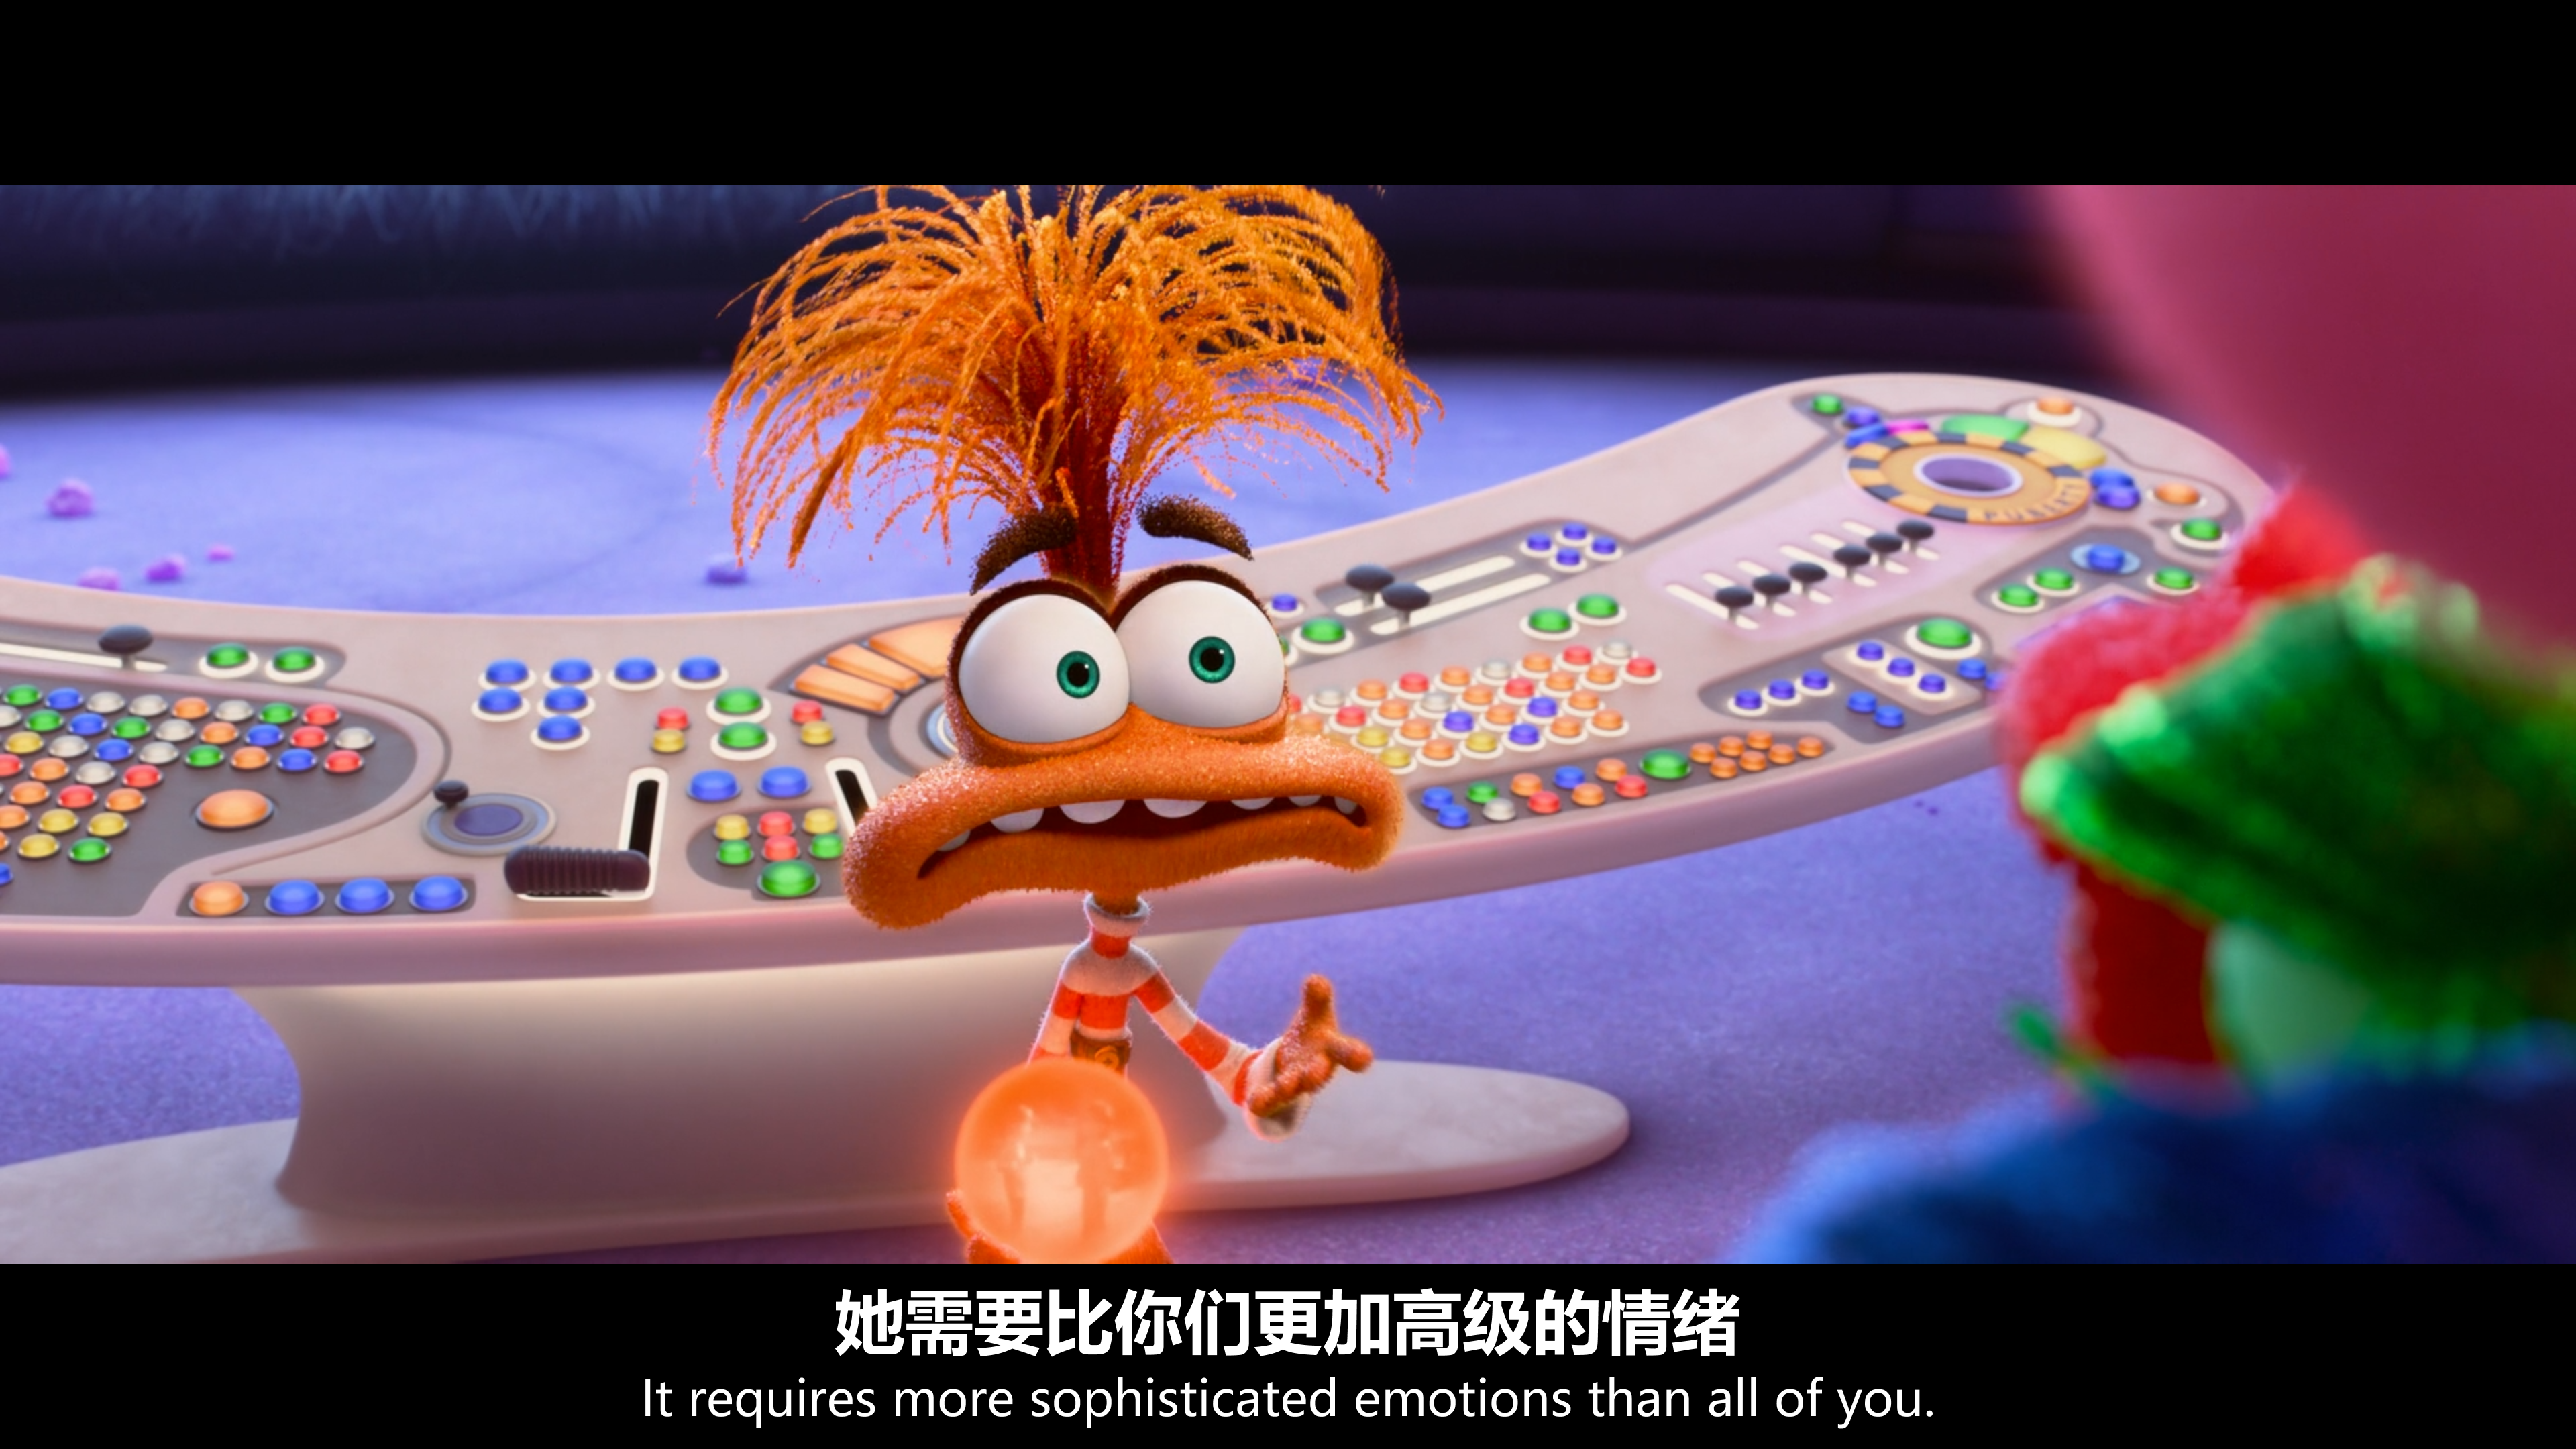
\includegraphics[width = .8\textwidth]{fig/长线思维和高级情绪.png}
    \caption{随着人物的成长，新的复杂的情绪开始出现}
\end{figure}
从心理学角度看，焦虑情绪的出现是前瞻性思维、风险评估等高级认知功能发展的结果。
她存在的首要意义，是帮助莱莉适应更复杂的社会环境，例如剧情中的高中冰球训练营。
她不是敌人，而是一个被过度激活的自我保护机制。正如在电影中提到：“怕怕负责保护我们免受看得见的伤害，而焦焦负责保护我们免受看不见的伤害”。

这让我想起了我的高复经历。
第一年高考失利，我选择复读。
在那一刻，我大脑总部的焦焦也夺取了控制权。
她有充分的理由：“我们失败过一次，绝对不能再失败。”

于是，她开始疯狂地为未来规划。我将每次模拟考试的成绩看得无比重要。这完全印证了埃利斯的ABC理论。

\begin{itemize}
    \item A (激发事件)： 某次模拟考的数学大题卡住了，或者总分比上次低了十分。

    \item B (信念系统)： 这是焦焦的主战场。她立刻激活了我的非理性信念：“这次考不好，就意味着我高考也考不好。”“我绝对不能犯任何错误。”“我完了，我的未来一片黑暗。”

    \item C (情绪与行为后果)： 极度的焦虑、恐慌，以及随之而来的失眠。
\end{itemize}

我的大脑在深夜复盘时，头脑中不断闪过高考失利的样子，模拟自己再次失败的窘境。
这是焦焦试图通过想象最坏的未来来控制未来。
\begin{figure}[H]
    \centering
    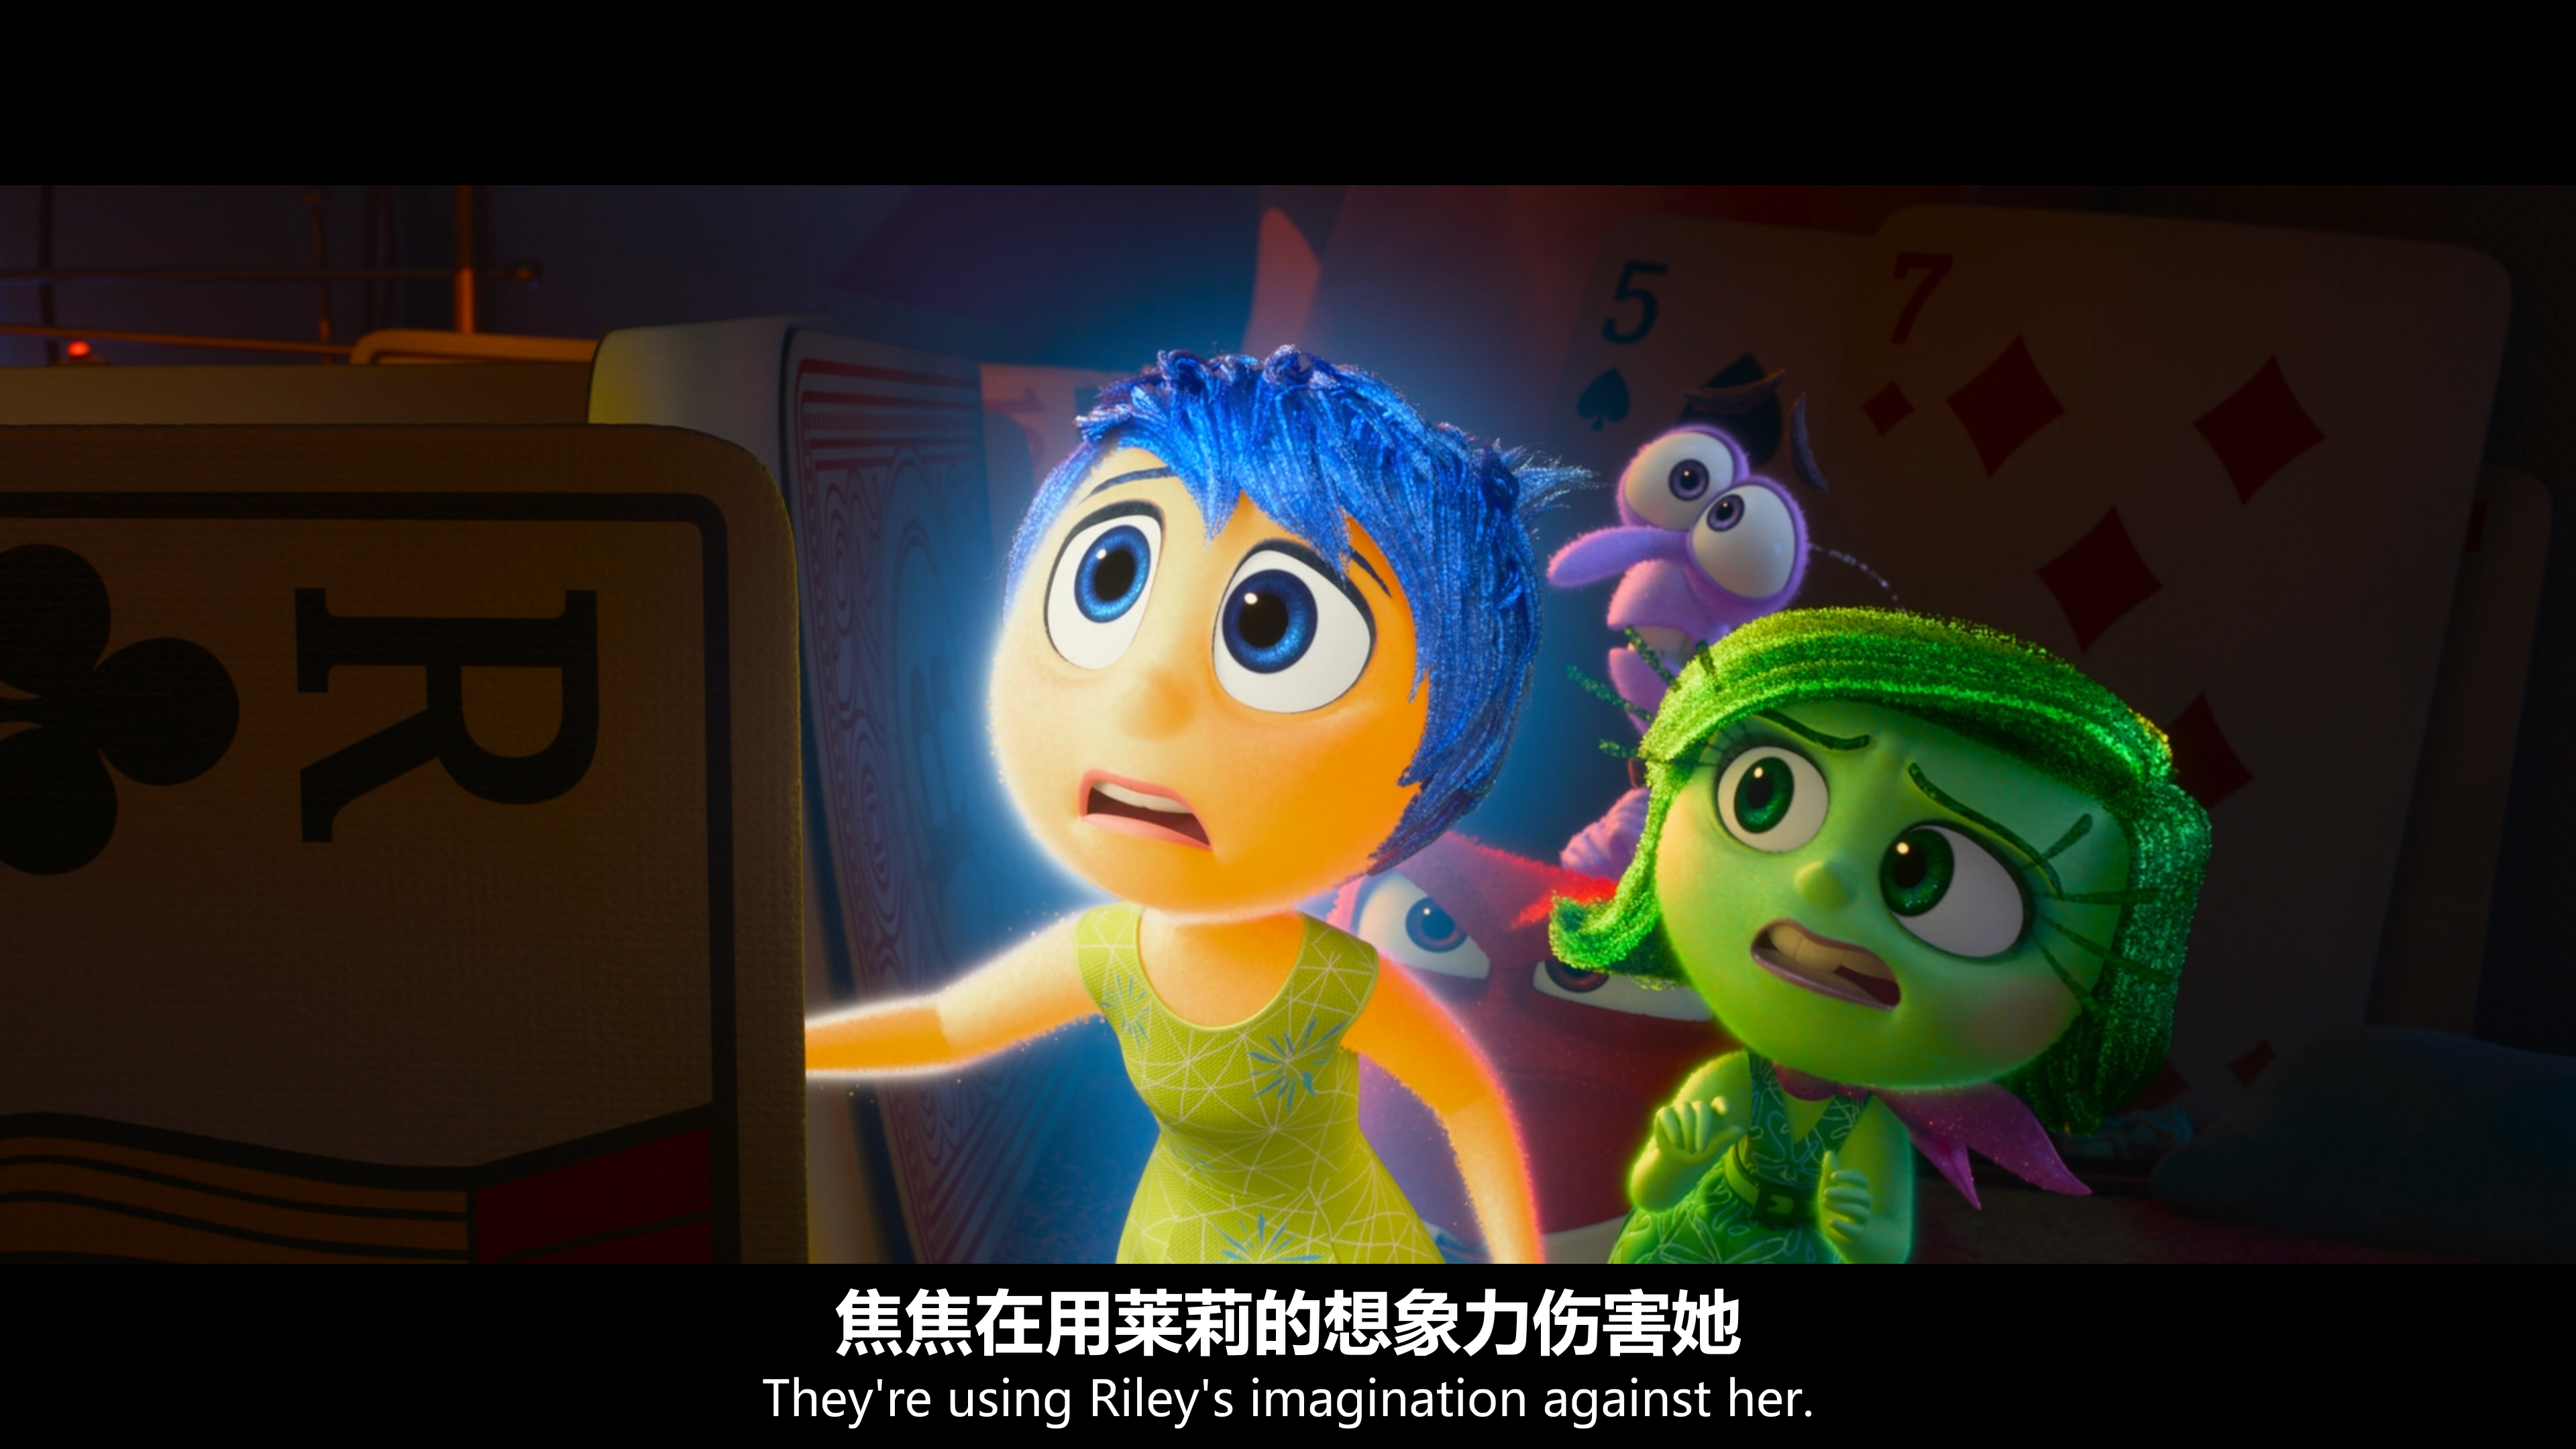
\includegraphics[width = .8\textwidth]{fig/折磨.png}
    \caption{过度的焦虑通过想象构建出不美好的未来}
\end{figure}
她构建了一个基于恐惧的、不正确的、极度不自信的自我，即“我是一个失败者”或“我是一个即将再次失败的人”。

\begin{figure}[H]
    \centering
    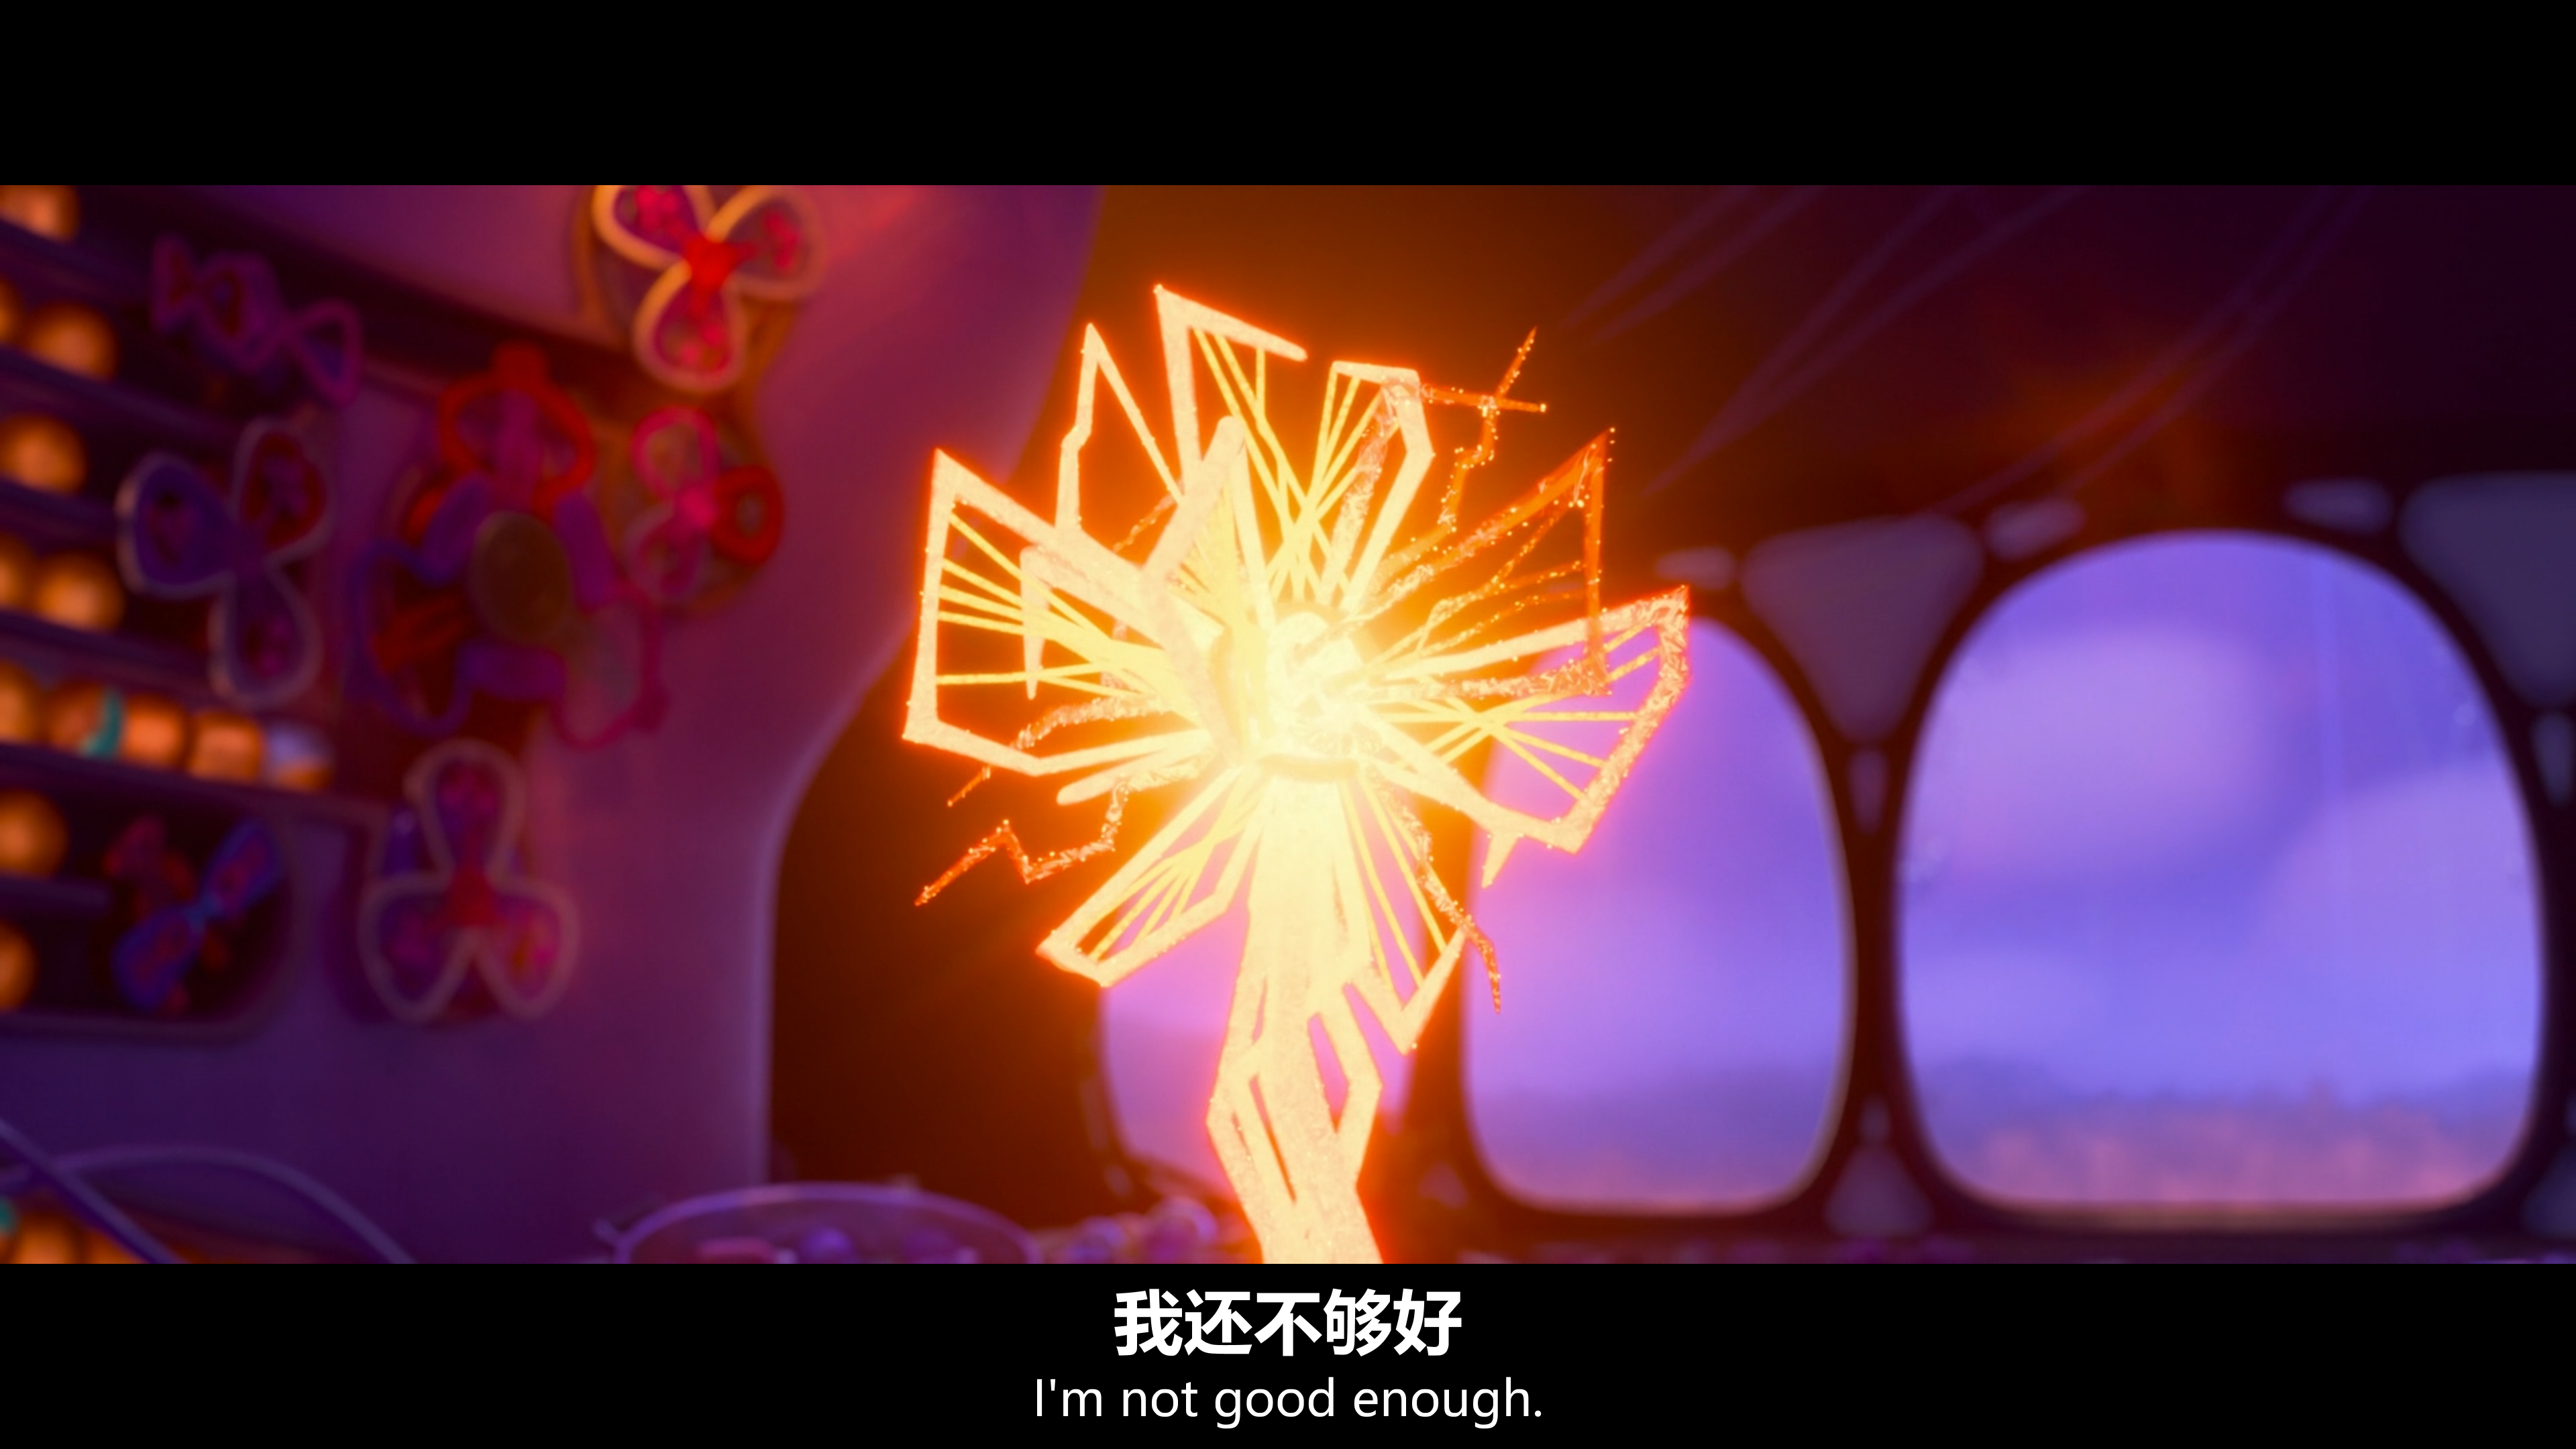
\includegraphics[width = .8\textwidth]{fig/诞生了焦虑的信念.png}
    \caption{蓝色的“好人”信念被焦虑的信念替代}
\end{figure}

\section{社交中的模仿}
焦焦的计划需要情报和执行。这时，阿慕和阿尬就成了她的左膀右臂。

阿慕的功能是扫描环境，找出威胁或榜样。她看到了瓦尔的优秀，于是焦焦立刻制定了计划：“模仿她，成为她，我们就能成功。”

这与我的高考语文作文经历如出一辙。我的目标是得到高分。而当时，我发现辞藻华丽的作文更可以拿高分。
于是，我开始盲目学习，阅读很多当时根本读不懂的哲学书目当作自己的人设，并在作文中不断引用那些晦涩的人名和概念，
将那些华丽的辞藻生硬地堆砌到自己的文字中。我放弃了自己真实的思考和感受，试图扮演一个高分考生。

而结果就是，我写出了一篇没有灵魂，没有自我思考的作文。

这更让我想起了我的初中岁月。我不善言辞，说了许多不合时宜的话，导致同学都不怎么理我。这个情境，激活了我对归属感的强烈渴求。

我大脑中的焦焦开始疯狂工作：“你必须取得他们的友谊！”
阿慕则指向那些受欢迎的同学：“看，他们是那样说话的！” 于是，我迫切地想和他们说更多的话，试图模仿那些“受欢迎”的样子。

但这种模仿是僵硬的、焦虑的。正如班杜拉的观察学习理论所示，我只“观察”了行为，却没有真正理解背后的认知和情境。我的模仿是拙劣的，反而说了更多错话。

每当我说错话时，阿尬就冲上控制台，拉下紧急制动。这种社死的体验是如此痛苦，以至于焦焦更加疯狂地制定补救措施，导致越说越错，最后闹得一地鸡毛。

在那个阶段，我和莱莉一样构建了一个虚假的、向外求索的自我，那就是：“我是一个模仿者”、“我是一个渴望被接纳却总在犯错的人”。

\section{当焦虑被按下暂停键}
转折点发生在莱莉被罚下场的两分钟，而这2分钟的处罚下场反而为莱莉点了暂停。

在赛场上，她被焦焦推着不断向前，没有喘息之机。而在这两分钟里，她被物理隔离了。

焦焦的计划导致了灾难性后果，莱莉因此在比赛中抛弃和伤害了曾经的朋友，也因为撞人而犯规被罚下场。那个焦虑的自我彻底失败了。

这与我初中经历的结局十分相似。在经历和品味了那一地鸡毛之后，我终于放下了这种焦虑。这种放下，并不是一个轻松的主动选择，它更像是一种阿丧的接管。

焦焦的能量耗尽了，阿尬的警报拉得太多次以至于麻木了。这种倦怠让我停止了徒劳的模仿和社交。

而正是在这个暂停期，在我不再疯狂地向外看时，我才终于有机会向内审视自我，仔细检查自己说话方式的问题。

这呼应了埃里克·伯恩的PAC理论。
在焦焦和阿尬的控制下，我一直处于一种焦虑的“儿童”（C）状态，渴望“父母”（P）状态的权威的认可。

而当我暂停时，我内心的“成人”（A）状态终于上线了。它开始客观地分析数据：“我说了什么？”“为什么不合时宜？”“我真实的想法是什么？” 正是这个“成人”状态的启动，
让我最终找到了真实的社交方式，取得了大家的信任。

\section{顿悟与重建——自我是一个复杂的融合}
如果说初中的暂停是成人状态的觉醒，那么高复时期的顿悟，则是一次彻底的自我意识的重建。

在我高复最焦虑的阶段，我遇到了一位心态很好的伙伴。他像是一面镜子，让我看到了活在焦虑之外的另一种存在方式。

这最终让我知道：一个人不是由自己的这些糟糕的记忆，和迫害自己的想象力决定的，而是由自己接下来需要走的路，自己想要成为什么人而决定的。

这句话，就是我对《头脑特工队2》结局的理解。

焦焦试图用第一次高考失利的糟糕回忆和幻想中再次失利的迫害自己的想象力来定义我，试图在自我意识的土地上，种下我不够优秀的信念。

而我的顿悟，是主动从焦焦手中夺回了控制权。我没有否认高考失利这个记忆，但我拒绝让它定义我的全部。

这正是莱莉在电影结尾所做的。她找回了被流放的“我是个好人”这个自我，但她也没有抛弃焦焦带来的新认知。

她最终的自我意识，不再是单一的颜色，而是一个复合。它是一个包含了所有经历、所有情绪、所有信念的、更庞大、更复杂的结构。

\begin{figure}[H]
    \centering
    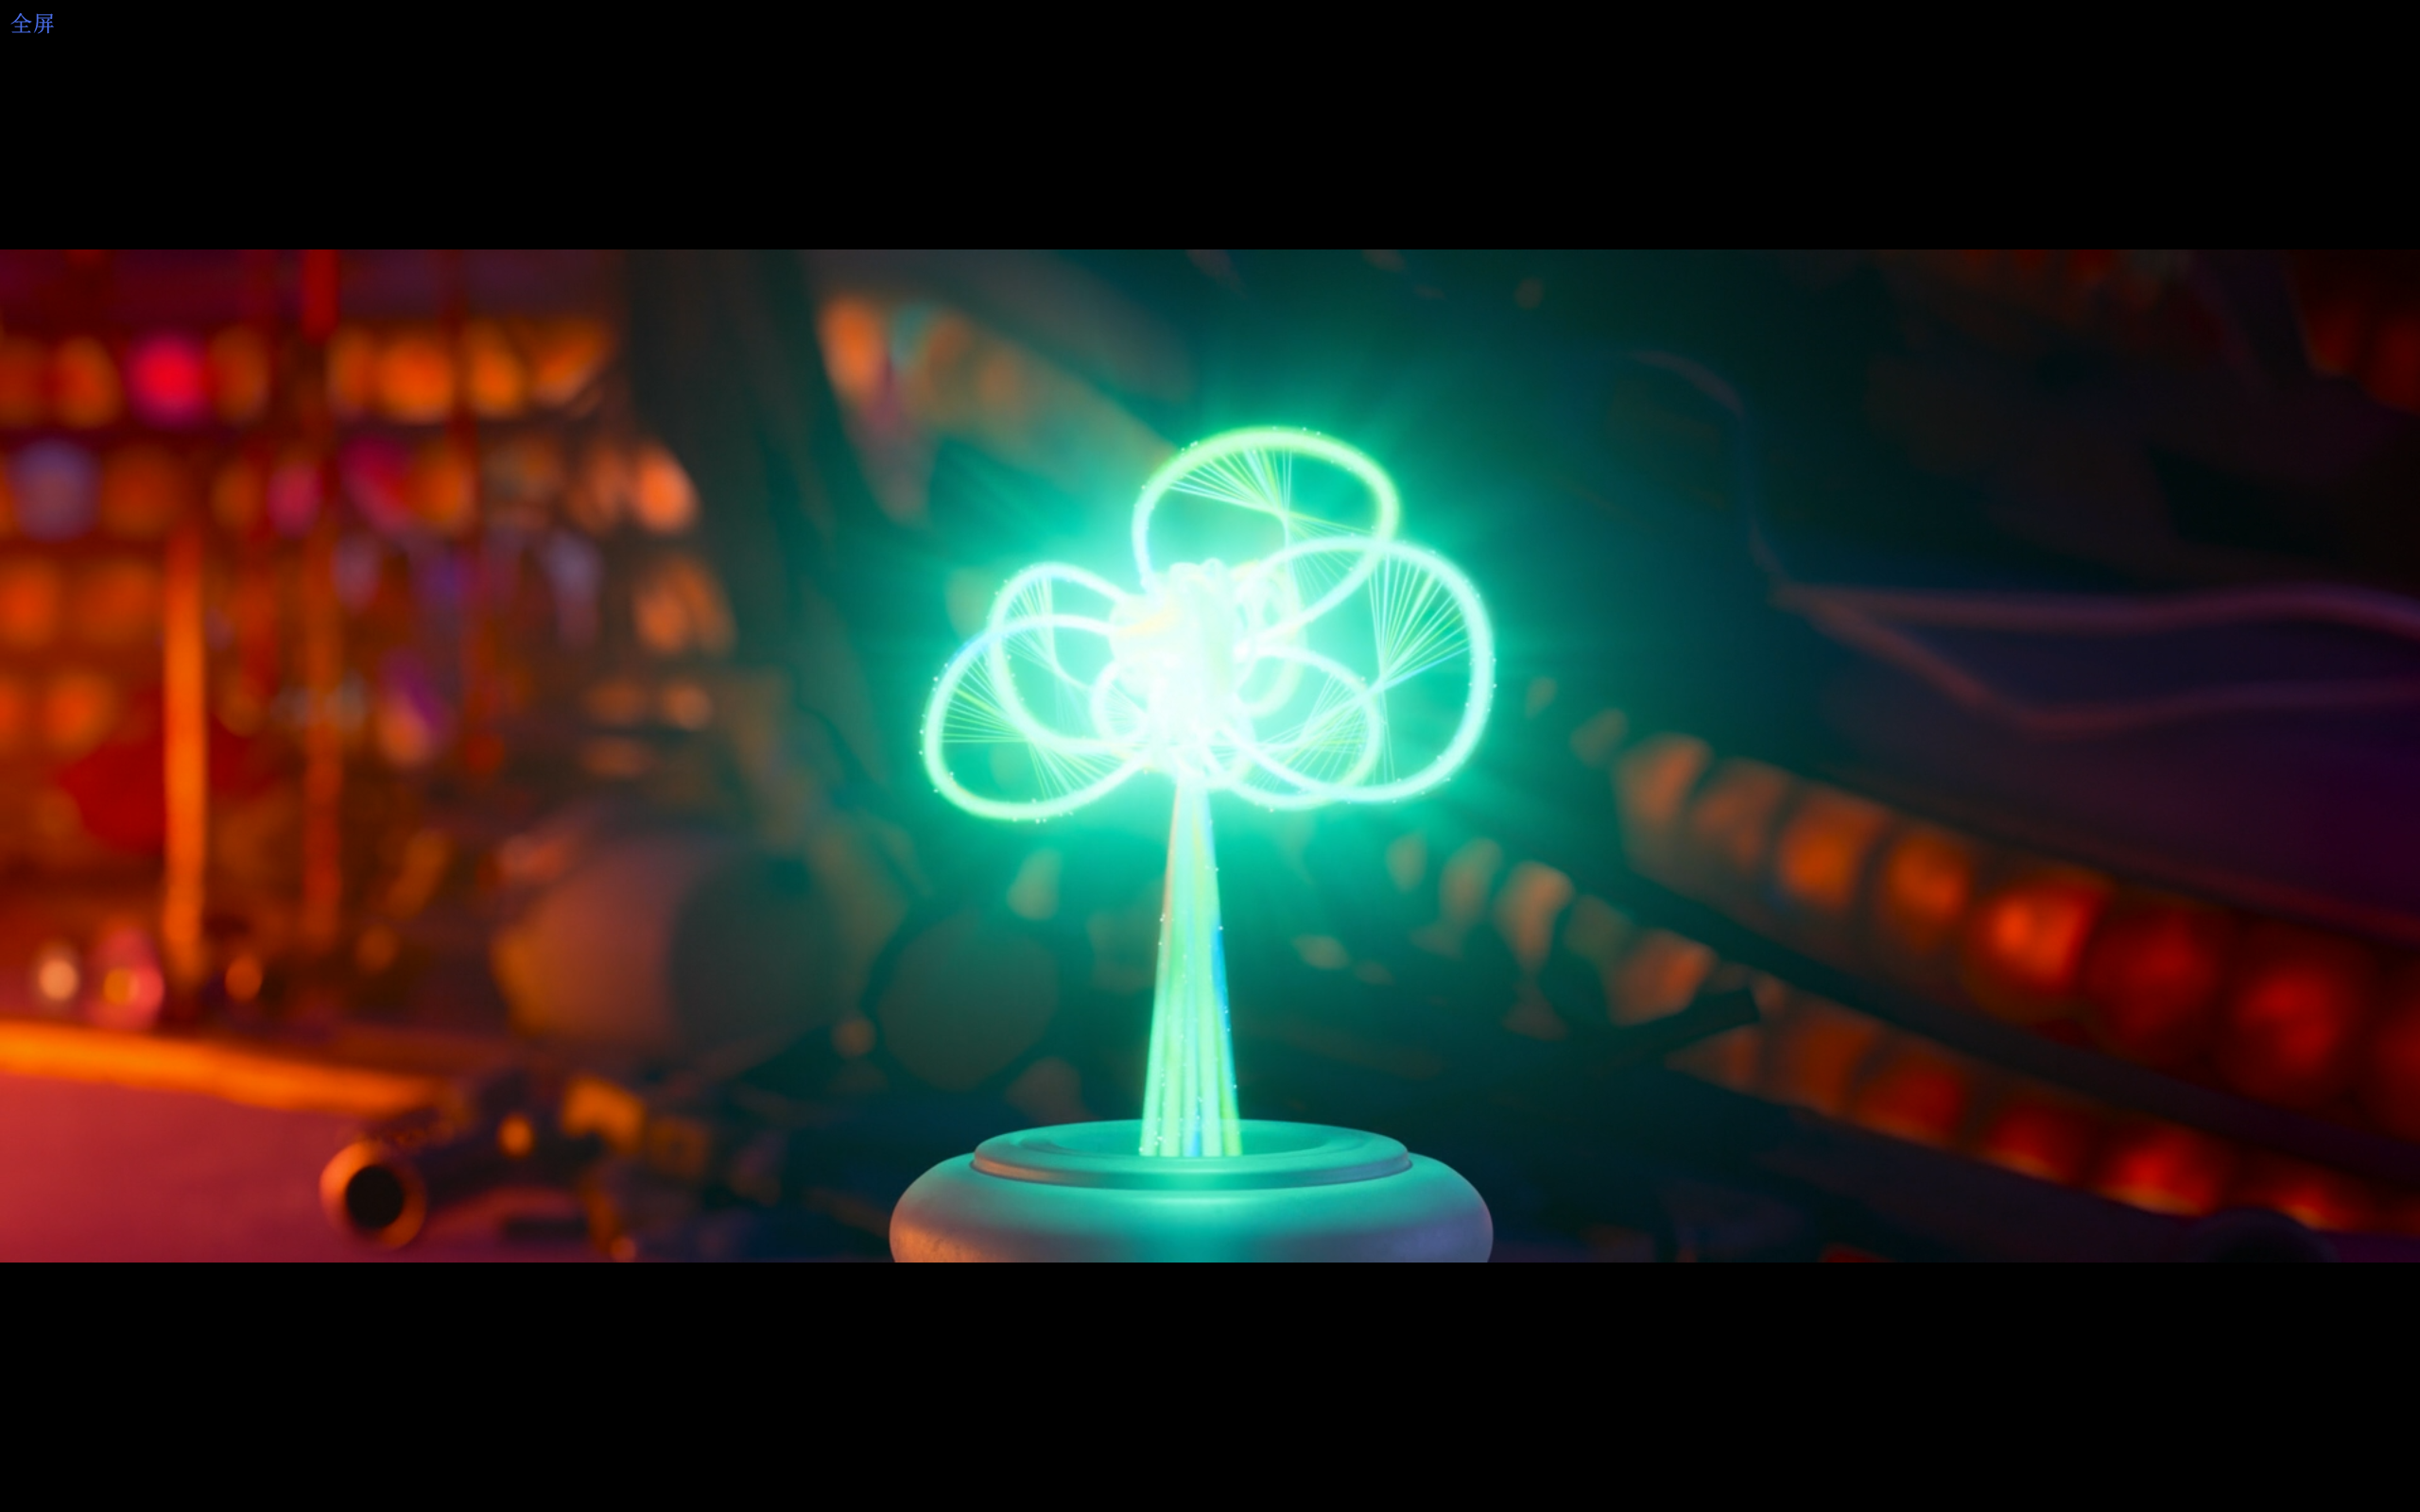
\includegraphics[width = .8\textwidth]{fig/复合.png}
    \caption{一颗复合的信念树，定义了完整的个体}
\end{figure}

这个新的自我意识是：
“我是一个好人。”
“我也是一个会焦虑的人。”
“我是一个重视友谊的人。”
“我也是一个有时会嫉妒他人的人。”
“我是一个经历过失败的人。”
“我更是一个正在为未来而战的人。”

这也和其他的结局“包饺子”的好莱坞大片形成了对比，进一步深化了主题。
\section{情绪的信使功能——理解情绪的信息能更好的调节情绪}
《头脑特工队2》除了探讨自我意识的构建，更给我带来了关于如何认识情绪与调节情绪的深刻启示。

在很长一段时间里，我们习惯于将情绪简单地二元对立：乐、喜是“好情绪”，而焦、丧、尬是“坏情绪”。我们对待“坏情绪”的方式，就像莱莉的旧团队对待焦焦她们一样——试图排斥、压抑、驱逐。
但电影清晰地揭示了：每一种情绪都是一个信使，它们的存在本身不是问题，而是来传递关键信息的

焦焦提醒我们潜在的风险；
阿慕让我们看清自己的渴望与差距；
阿尬在校准我们的社交边界；
阿丧则在能量耗尽时强制我们休息。
认识情绪的第一步，就是停止将它们视为敌人，而是去理解它们带来的信息。

而在调节情绪方面，电影也展示了两种最常见的错误策略：
\begin{enumerate}
    \item 情绪压抑：就像旧情绪们被焦焦打包流放一样。
    这种压抑并不会让情绪消失，它们只会在“意识后端”积压，最终以更具破坏性的方式发展，
    比如莱莉最后经历的焦虑风暴中爆发。
    \item 情绪主宰：即任由一种情绪完全接管控制台。
    这导致了莱莉的灾难性行为，即她所有的行动都基于恐惧和最坏的打算，完全偏离了她本来的价值观，比如她在选择队伍的时候抛弃了旧时的朋友。
    这正是我在高复时被阿焦支配，写出没有灵魂的作文的翻版。
\end{enumerate}

真正的情绪调节，不是压抑，更不是放任，而是电影结尾所展现的调和和整合。

这正是我在PAC理论中学到的“成人”状态的核心功能。我们的自我不应该是任何一种情绪的奴隶，
而应是控制台前的指挥官。当阿焦冲上来说“我们完蛋了！”时，成人自我的工作不是把她扔出去，
而是倾听她，安抚她：“我收到你的警报了，谢谢你提醒我这件事很重要。现在，让我们看看具体的数据，制定一个可行的计划。”

这种调节，是学会从“我就是很焦虑”的情绪融合转变为“我觉察到了焦虑的情绪”的情绪觉察。
我们承认风暴的存在，但我们握紧方向盘，利用风暴的能量，而不是被它掀翻。
我们接纳所有信使，但“我是谁”以及“我该怎么做”，最终由“自我”这个掌舵者来决定。

\section{接纳一切，然后走向未来}
这部电影让我认识到构成自我意识这个世界上最美好的东西的，恰恰是所有的信念，无论是好是坏。

焦焦不是敌人，她教会我们规划；阿慕不是原罪，她为我们指出榜样；阿尬不是羞耻，她为我们校准社交边界；阿丧不是堕落，她为我们提供必要的喘息。

我的初中经历，让我学会了在阿尬和焦焦的噪音中，启动“成人”状态的反思。
我的复读经历，让我学会在焦焦的灾难化预言中，坚守一个面向未来的、自己选择的信念。

健康的“自我”，不是一个没有焦虑、没有嫉妒的“纯金”自我，而是一个认识到自己是一个“复合体”的自我。
我们承认内心的风暴，接纳所有的情绪，然后对自己说：“你们都在。但我，才是我人生的掌舵者。”
\end{document}